\documentclass[UTF8]{ctexart}
\usepackage{algpseudocode}
\usepackage{algorithm}
\usepackage{amsmath}
\usepackage{subcaption}
\usepackage{graphicx}
\usepackage[bottom=6em]{geometry}
\usepackage{lmodern}
\usepackage{listings}
\usepackage{xcolor}

\ctexset{ section = { format={\Large \bfseries } } }

\pagestyle{empty}

\begin{document}

\section*{Task 1: Phong Illumination}

按照课件给出的公式计算即可。

\begin{figure}[htbp]
    \begin{subfigure}[b]{0.49\textwidth}
        \centering
        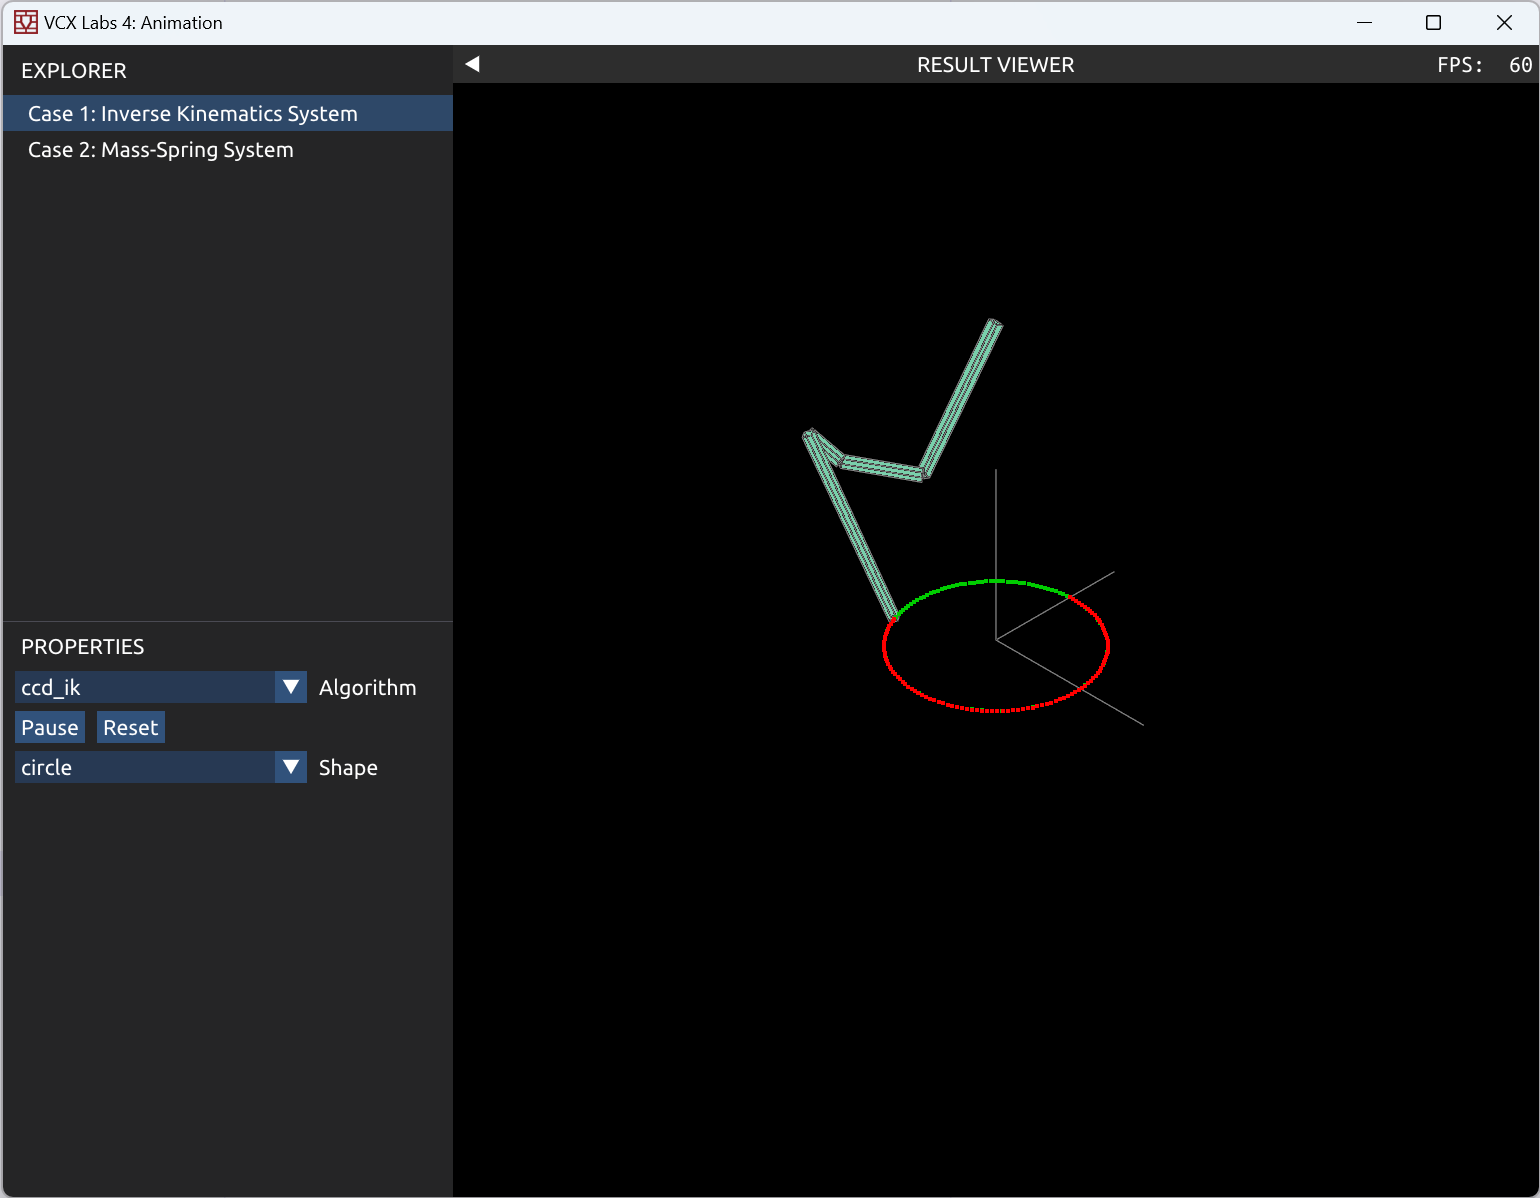
\includegraphics[width=\textwidth]{images/1-1.png}
        \caption{Phong 光照模型}
    \end{subfigure}
    \hfill
    \begin{subfigure}[b]{0.49\textwidth}
        \centering
        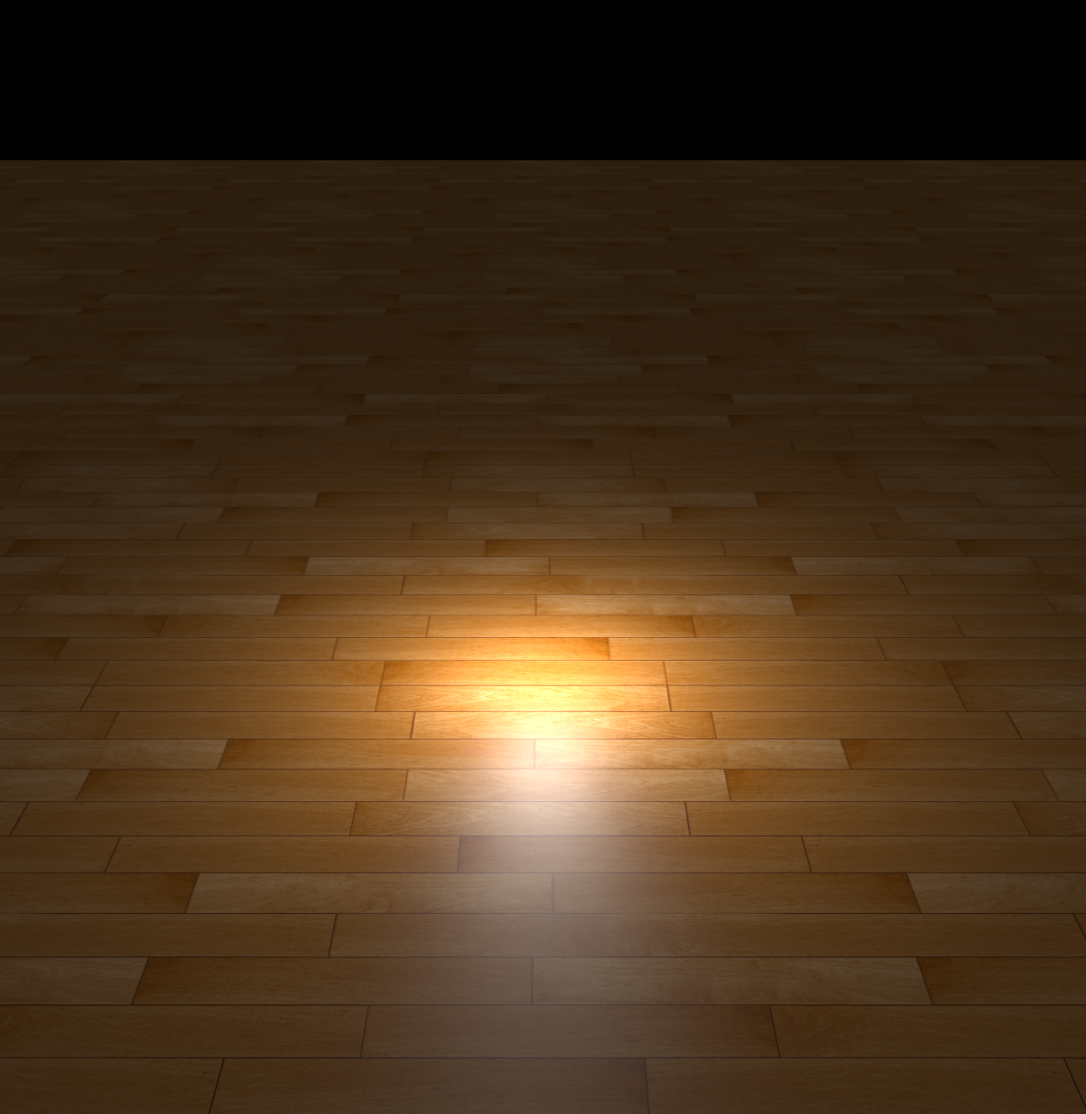
\includegraphics[width=\textwidth]{images/1-2.png}
        \caption{Blinn-Phong 光照模型}
    \end{subfigure}
    \caption*{Task 1}
\end{figure}

\begin{enumerate}
    \item 顶点着色器和片段着色器是渲染管线的前后两个部分。顶点着色器处理顶点属性,在经过一系列操作后再由片段着色器处理每个像素的颜色。管线的每个阶段以前一个阶段的输出作为输入,顶点着色器的输出会经由中间阶段处理后成为片段着色器的输入。
    \item 这行语句用于在像素不透明度过小时忽略该像素。不能使用 \texttt{if (diffuseFactor.a == 0.) discard;} 是因为浮点数一般需要处理误差,而且透明度较高的情况可能是一些图像的边缘部分,本来应该被忽略。
\end{enumerate}

\section*{Task 2: Environment Mapping}

在计算立方体贴图的位置时,应当移除观察矩阵的位移部分,保留旋转部分,并且设置其位置的 z 值为 1,确保它在所有物体的后方。计算环境映射时,将视线方向按物体表面的法向做反射,从立方体贴图中采样。

\begin{figure}[htbp]
    \begin{subfigure}[b]{0.49\textwidth}
        \centering
        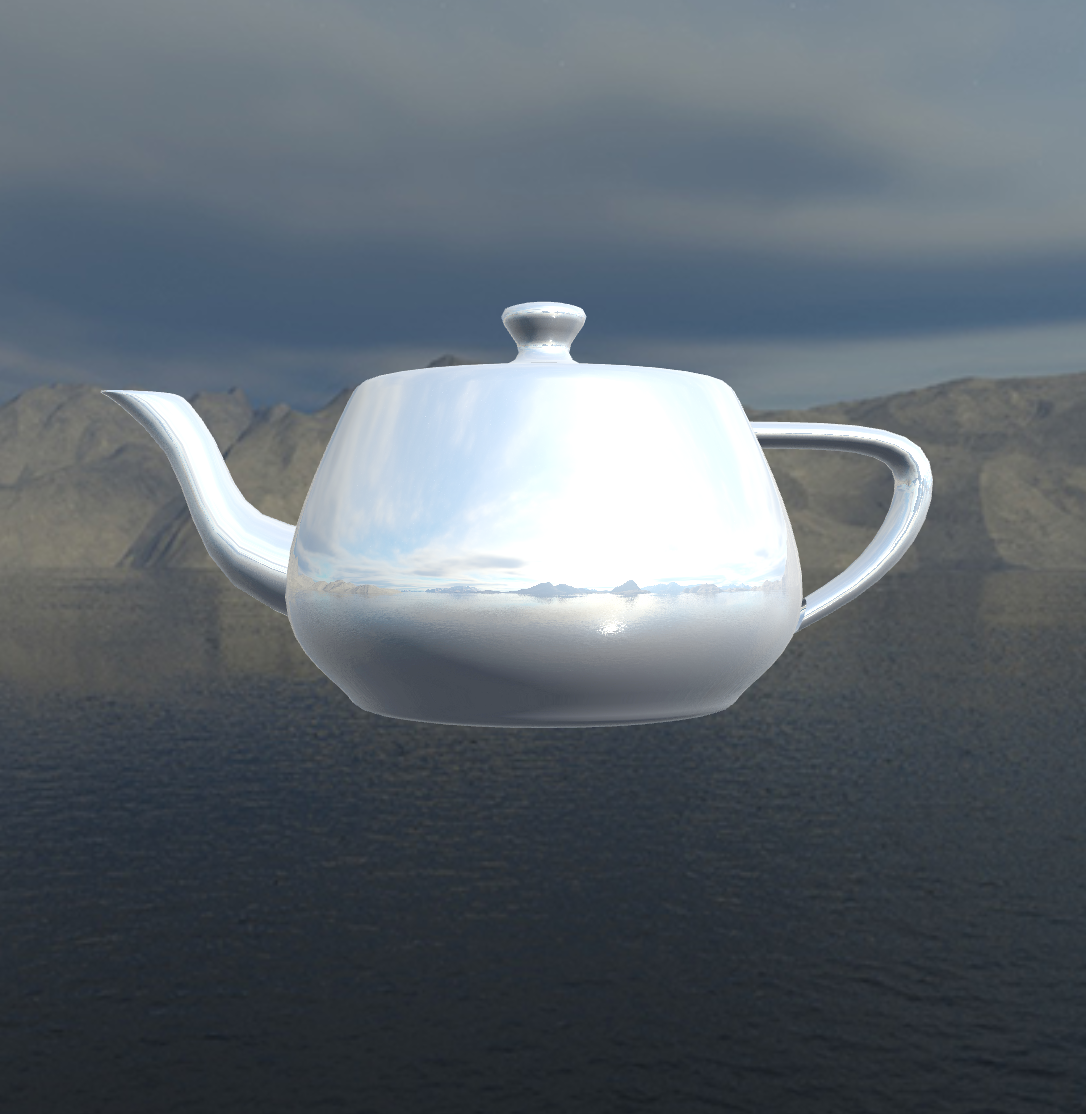
\includegraphics[width=\textwidth]{images/2-1.png}
        \caption{teapot 场景}
    \end{subfigure}
    \hfill
    \begin{subfigure}[b]{0.49\textwidth}
        \centering
        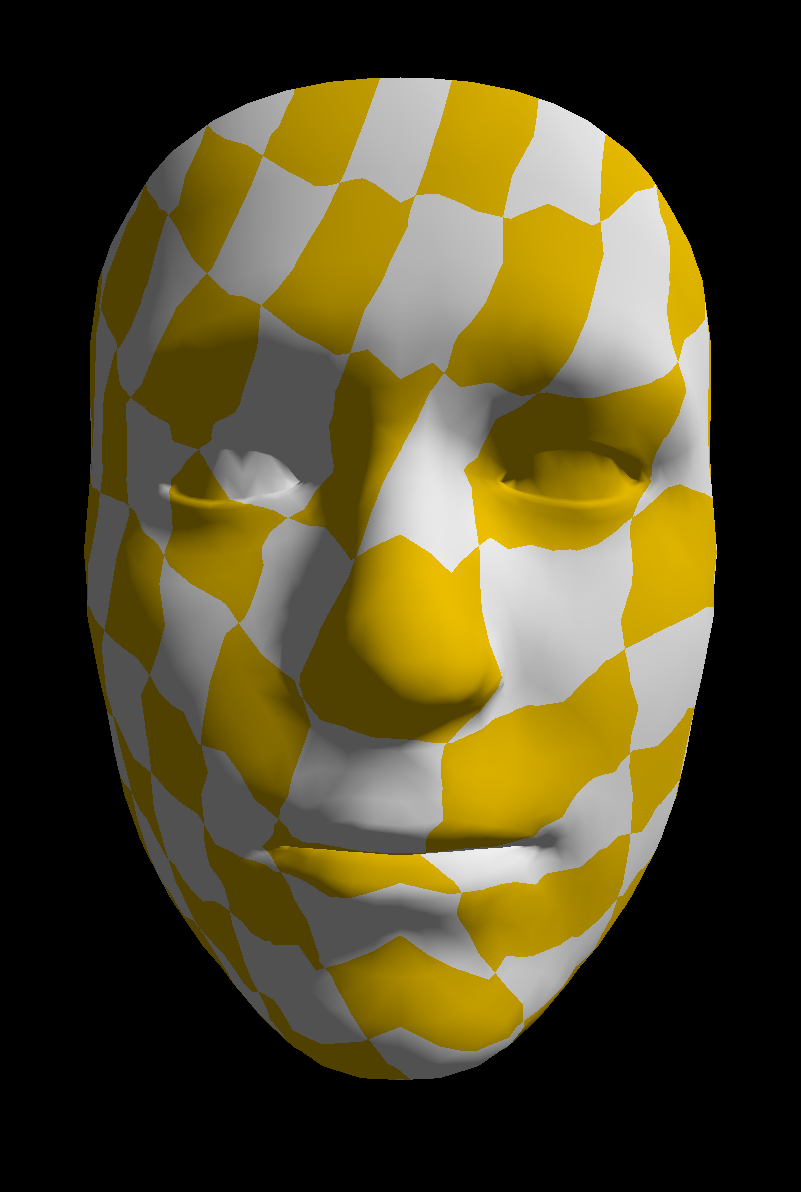
\includegraphics[width=\textwidth]{images/2-2.png}
        \caption{bunny 场景}
    \end{subfigure}
    \caption*{Task 2}
\end{figure}

\section*{Task 3: Non-Photorealistic Rendering}

将光线方向与法向夹角的余弦上取整到 $1/4$ 的整数倍,按照这个值来对冷色和热色进行插值。

\begin{figure}[htbp]
    \begin{subfigure}[b]{0.49\textwidth}
        \centering
        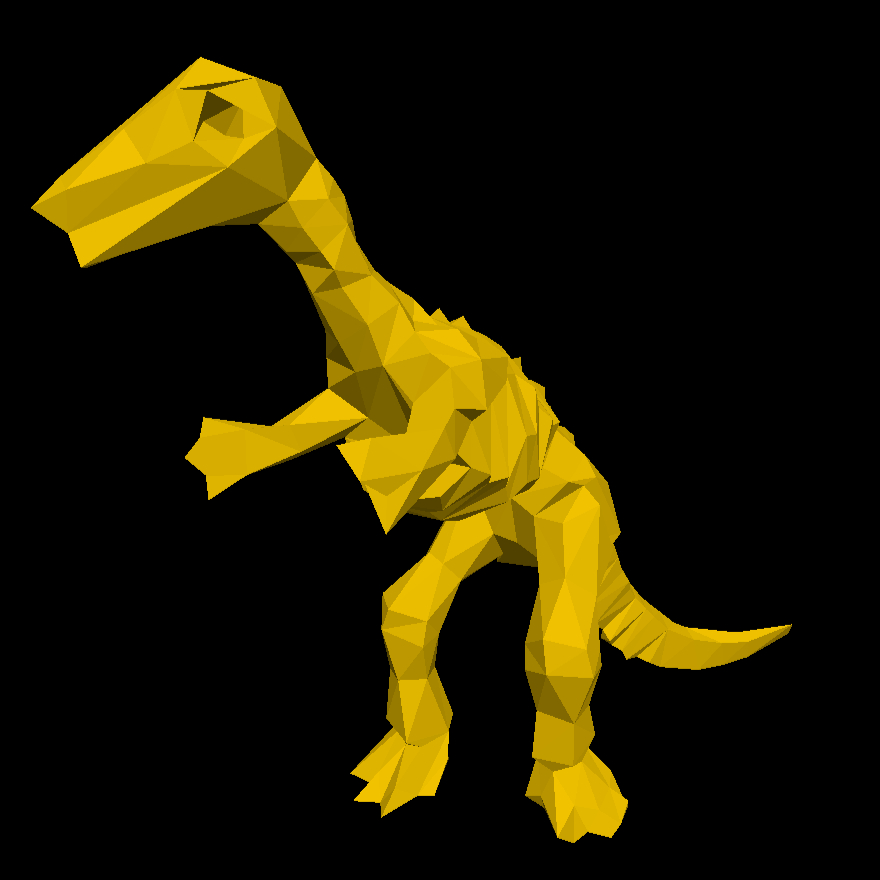
\includegraphics[width=\textwidth]{images/3-1.png}
        \caption{teapot 场景}
    \end{subfigure}
    \hfill
    \begin{subfigure}[b]{0.49\textwidth}
        \centering
        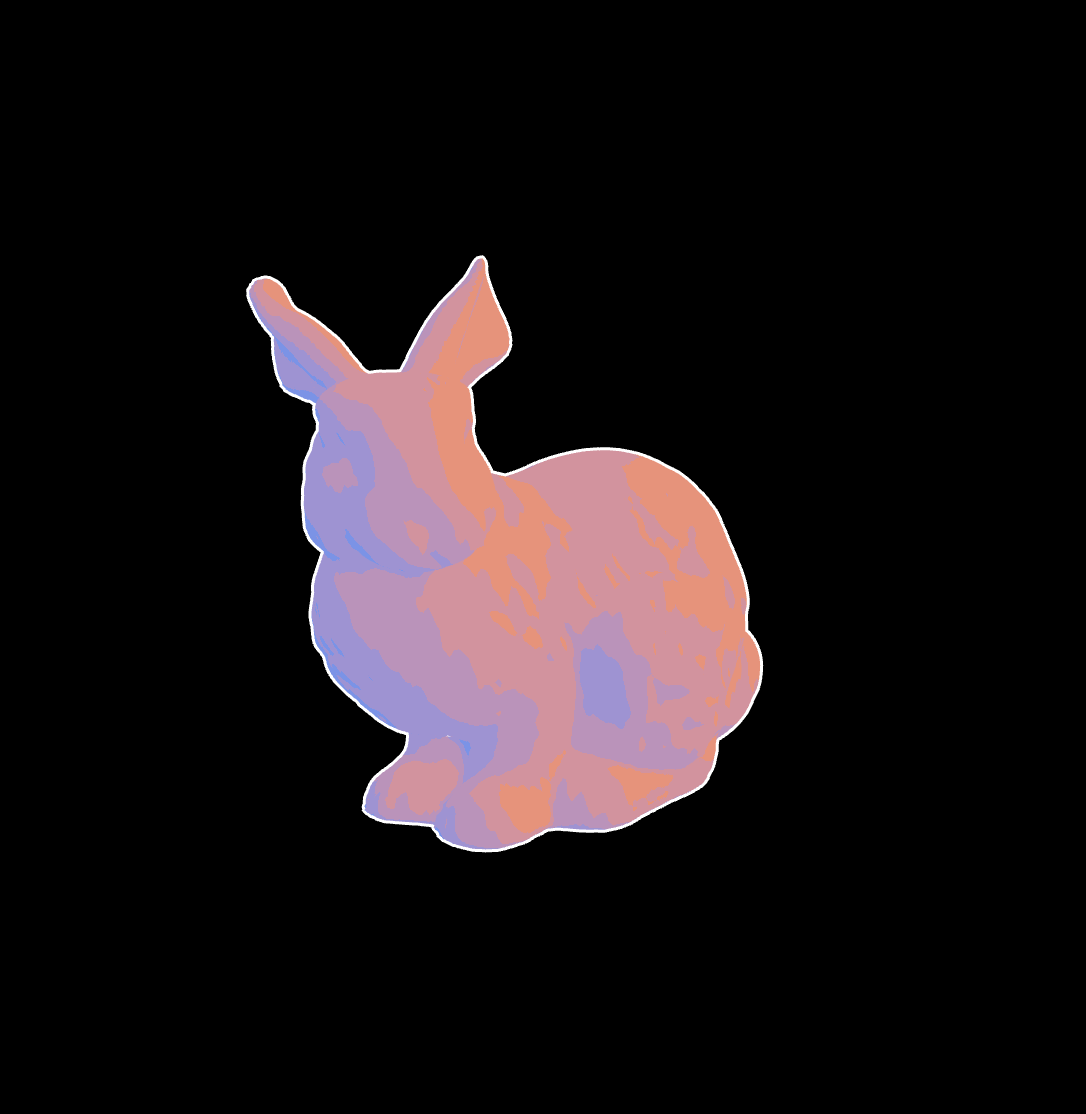
\includegraphics[width=\textwidth]{images/3-2.png}
        \caption{bunny 场景}
    \end{subfigure}
    \caption*{Task 3}
\end{figure}

\begin{enumerate}
    \item 函数使用 \texttt{glCullFace(GL\_FRONT); glEnable(GL\_CULL\_FACE);} 这两行代码剔除了正面,随后进行背面的渲染。然后反过来剔除背面,渲染正面,实现了分别的处理。
    \item 世界坐标中沿着法向移动会导致在摄像机的位置看到的轮廓粗细不同。
\end{enumerate}

\section*{Task 4: Shadow Mapping}

我使用了第一题的 Blinn-Phong 光照模型。在获取深度信息时,使用 \texttt{texture} 函数从深度贴图中采样即可。

\begin{figure}[htbp]
    \begin{subfigure}[b]{0.49\textwidth}
        \centering
        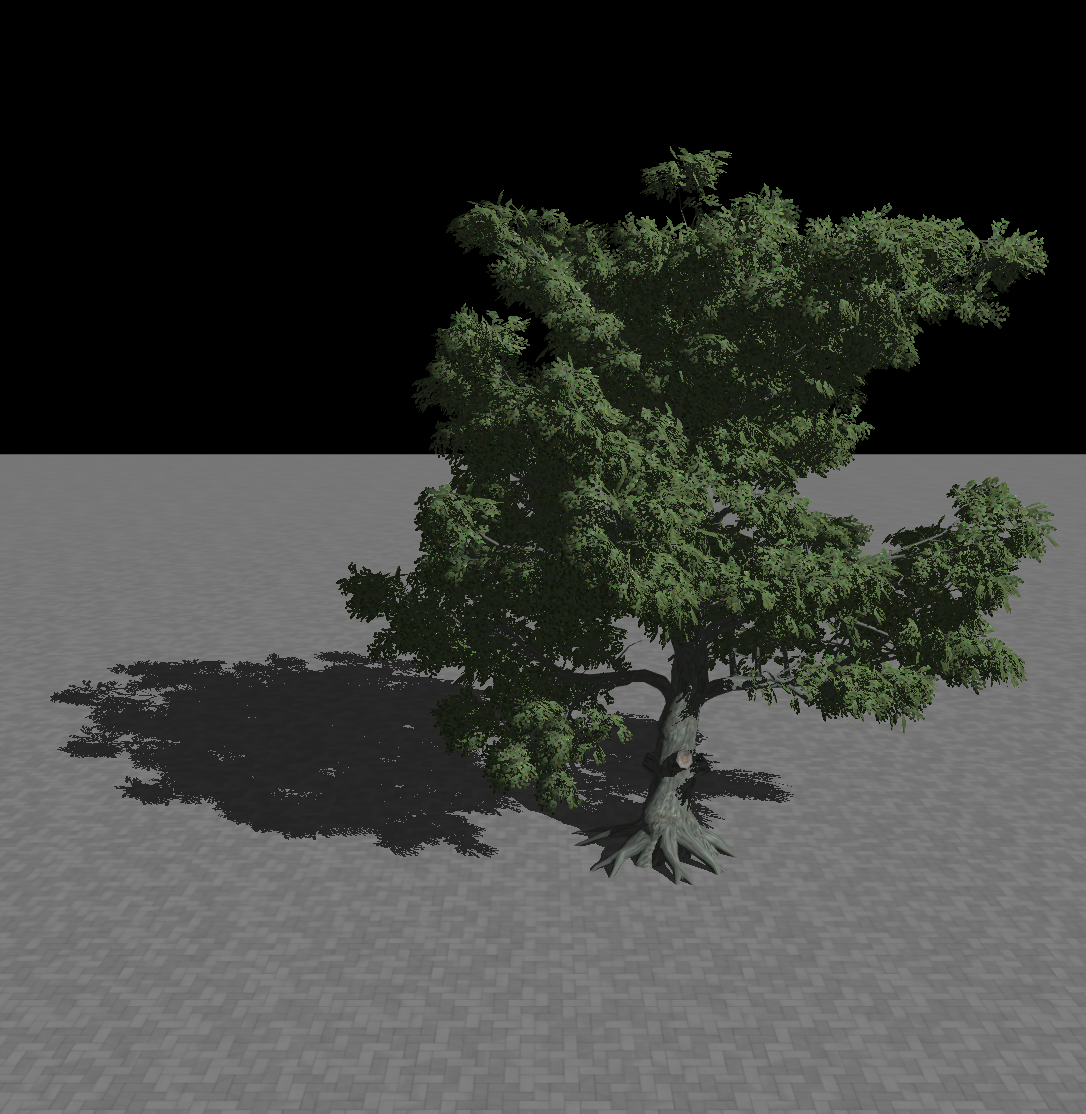
\includegraphics[width=\textwidth]{images/4-1.png}
        \caption{white oak 场景}
    \end{subfigure}
    \hfill
    \begin{subfigure}[b]{0.49\textwidth}
        \centering
        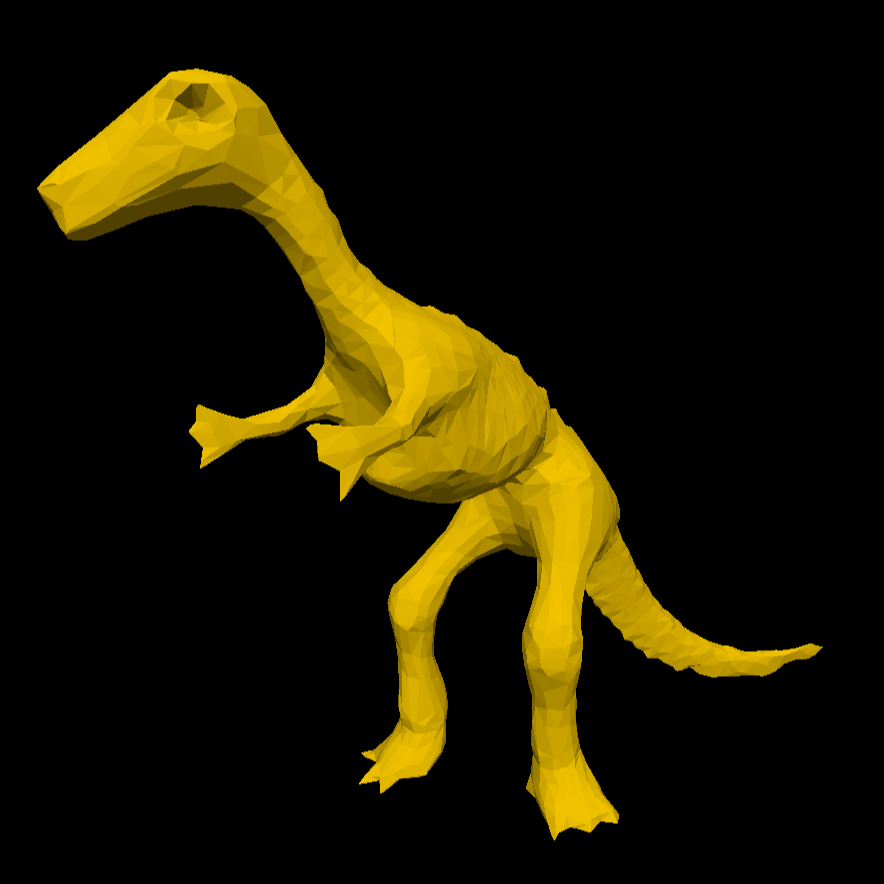
\includegraphics[width=\textwidth]{images/4-2.png}
        \caption{sponza 场景}
    \end{subfigure}
    \caption*{Task 4}
\end{figure}

\begin{enumerate}
    \item 有向光源应该使用正交投影矩阵,点光源应该使用透视投影矩阵。
    \item 实际上计算了在光源视角下的坐标(包括深度)。
\end{enumerate}

\section*{Task 5: Whitted-Style Ray Tracing}

光线和三角形求交的算法按照提供的论文实现。着色的部分类似第一题,环境光强度设为 $0.1$。阴影的部分从着色点向光源射出光线判断是否有不透明的物体即可。

\begin{figure}[htbp]
    \centering
    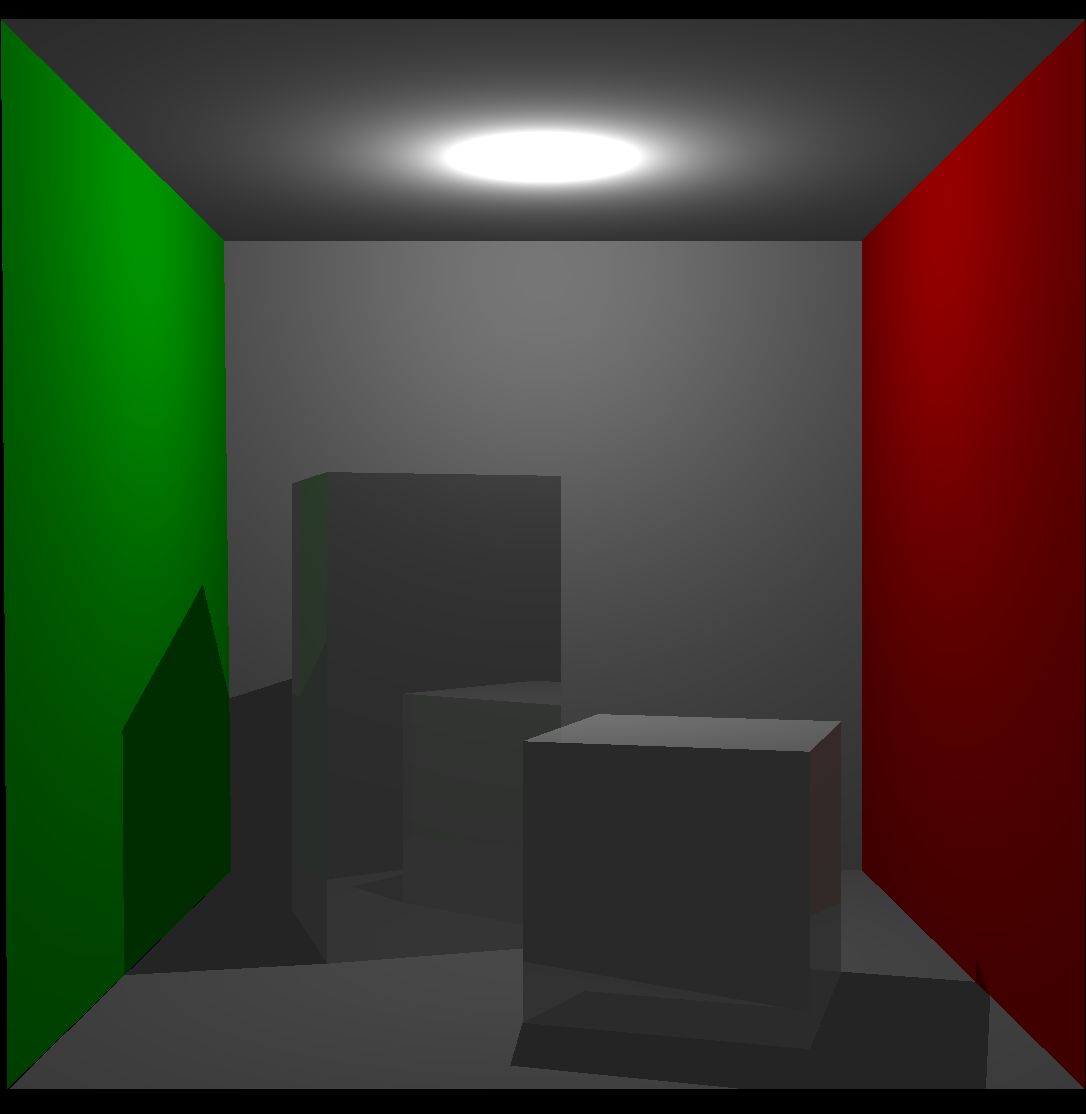
\includegraphics[width=0.8\textwidth]{images/5-1.png}
    \caption*{Task 5:Cornell Box 场景}
\end{figure}

光线追踪可以实现反射、折射等效果。在处理影子时,光栅化的渲染效果受限于深度贴图的分辨率,靠近观察阴影边缘可以发现明显的锯齿,而光线追踪由于本身原理不同,对于这类情况的处理与摄像机位置无关。

\end{document}